\documentclass[a5paper, 10pt]{article}

% Текст
\usepackage[utf8]{inputenc} % UTF-8 кодировка
\usepackage[russian]{babel} % Русский язык
\usepackage{indentfirst} % красная строка в первом параграфе в главе
% Отображение страниц
\usepackage{geometry} % размеры листа и отступов
\usepackage{listings}
\usepackage{color}

\geometry{
	left=12mm,
	top=25mm,
	right=15mm,
	bottom=17mm,
	marginparsep=0mm,
	marginparwidth=0mm,
	headheight=10mm,
	headsep=7mm,
	nofoot}
\usepackage{afterpage,fancyhdr} % настройка колонтитулов
\pagestyle{fancy}
\fancypagestyle{style}{ % создание нового стиля style
	\fancyhf{} % очистка колонтитулов
	\fancyhead[LO, RE]{Лабораторная работа № 4 } % название документа наверху
	\fancyhead[RO, LE]{Линейная фильтрация} % название section наверху
	\fancyfoot[RO, LE]{\thepage} % номер страницы справа внизу на нечетных и слева внизу на четных
	\renewcommand{\headrulewidth}{0.25pt} % толщина линии сверху
	\renewcommand{\footrulewidth}{0pt} % толцина линии снизу
}
\fancypagestyle{plain}{ % создание нового стиля plain -- полностью пустого
	\fancyhf{}
	\renewcommand{\headrulewidth}{0pt}
}
\fancypagestyle{title}{ % создание нового стиля title -- для титульной страницы
	\fancyhf{}
	\fancyhead[C]{{\footnotesize
			Министерство образования и науки Российской Федерации\\
			Федеральное государственное автономное образовательное учреждение высшего образования
	}}
	\fancyfoot[C]{{\large 
			Санкт-Петербург, 2024
	}}
	\renewcommand{\headrulewidth}{0pt}
}

% Математика
\usepackage{amsmath, amsfonts, amssymb, amsthm} % Набор пакетов для математических текстов
%\usepackage{dmvnbase} % мехматовский пакет latex-сокращений
\usepackage{cancel} % зачеркивание для сокращений
% Рисунки и фигуры
\usepackage[pdftex]{graphicx} % вставка рисунков
\usepackage{wrapfig, subcaption} % вставка фигур, обтекая текст
\usepackage{caption} % для настройки подписей
\captionsetup{figurewithin=none,labelsep=period, font={small,it}} % настройка подписей к рисункам
% Рисование
\usepackage{tikz} % рисование
\usepackage{circuitikz}
\usepackage{pgfplots} % графики
% Таблицы
\usepackage{multirow} % объединение строк
\usepackage{multicol} % объединение столбцов
% Остальное
\usepackage[unicode, pdftex]{hyperref} % гиперссылки
\usepackage{enumitem} % нормальное оформление списков
\setlist{itemsep=0.15cm,topsep=0.15cm,parsep=1pt} % настройки списков
% Теоремы, леммы, определения...
\theoremstyle{definition}
\newtheorem{Def}{Определение}
\newtheorem*{Axiom}{Аксиома}
\theoremstyle{plain}
\newtheorem{Th}{Теорема}
\newtheorem{Lem}{Лемма}
\newtheorem{Cor}{Следствие}
\newtheorem{Ex}{Пример}
\theoremstyle{remark}
\newtheorem*{Note}{Замечание}
\newtheorem*{Solution}{Решение}
\newtheorem*{Proof}{Доказательство}
% Свои команды
\newcommand{\comb}[1]{\left[\hspace{-4pt}\begin{array}{l}#1\end{array}\right.\hspace{-5pt} } % совокупность уравнений
% Титульный лист
\usepackage{csvsimple-l3}
\newcommand*{\titlePage}{
	\thispagestyle{title}
	\begingroup
	\begin{center}
		%		{\footnotesize
			%			Министерство образования и науки Российской Федерации\\
			%			Федеральное государственное автономное образовательное учреждение высшего образования
			%		}
		%		
		\vspace*{6ex}
		
		{\small
			САНКТ-ПЕТЕРБУРГСКИЙ НАЦИОНАЛЬНЫЙ ИССЛЕДОВАТЕЛЬСКИЙ УНИВЕРСИТЕТ ИТМО	
		}
		
		\vspace*{2ex}
		
		{\normalsize
			Факультет систем управления и робототехники
		}
		
		\vspace*{15ex}
		
		{\Large \bfseries 
			Лабораторная работа № 4
		}
\vspace*{2ex}
	{\Large \bfseries 
			
"Линейная фильтрация"
		}
\vspace*{2ex}
		
		{\normalsize
			по дисциплине Частотные методы
		}

	\end{center}
	\vspace*{20ex}
	\begin{flushright}
		{\large 
			\underline{Выполнила}: студентка гр. \textbf{R3238}\\
			\begin{flushright}
				\textbf{Нечаева А. А.}\\
			\end{flushright}
		}
		
		\vspace*{5ex}
		
		{\large 
			\underline{Преподаватель}: \textit{Перегудин Алексей Алексеевич}
		}
	\end{flushright}	
	\newpage
	\setcounter{page}{1}
	\endgroup}

\begin{document}
	\titlePage
	\pagestyle{style}
\newpage


\section{Задание. Спектральное дифференцирование}
 \subsection{Исходный график}
Рассмотрим сигнал $y=\sin (t)$ на промежутке $[-100; 100]$ (рисунок 1).

\begin{figure}[h!]
\center{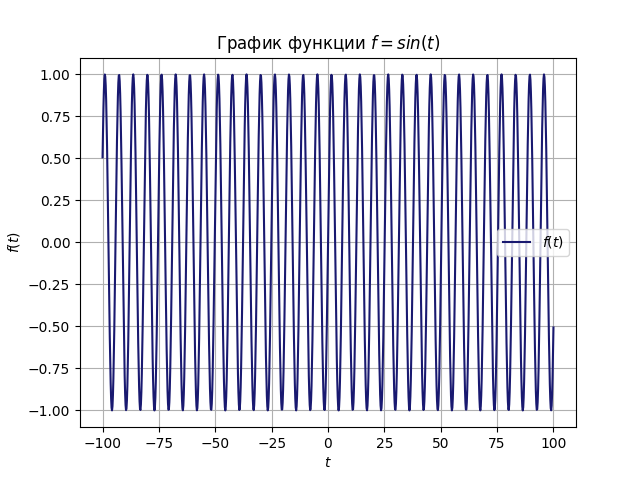
\includegraphics[width=1\linewidth]{pic1/sin_1.png}}
\caption{Исходный график $f= \sin(t)$.}
\end{figure}

Будем также рассматривать часть исходного графика на промежутке $[-10; 10]$ (рисунок 2) для большей наглядности.

\begin{figure}[h!]
\center{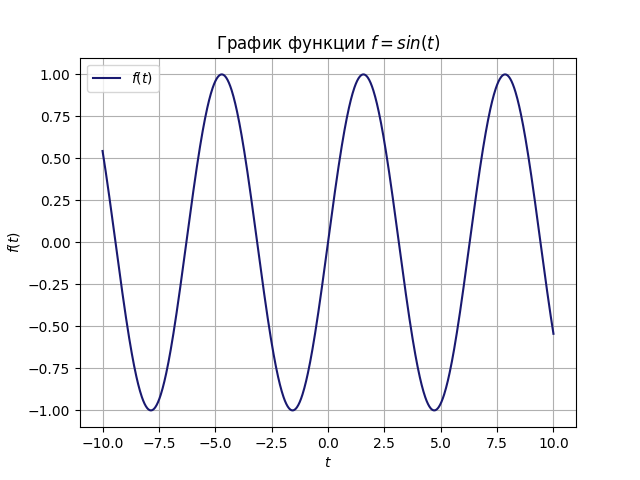
\includegraphics[width=1\linewidth]{pic1/sin_2.png}}
\caption{Часть исходный график $f= \sin(t)$.}
\end{figure}


\newpage
\subsection{Добавление шума}

Добавим к исходному графику функции небольшой шум вида $$a \cdot \left( rand (size(t)) - 0.5  \right)$$ результат представлен на рисунках 4 и 5.

\begin{figure}[h!]
\center{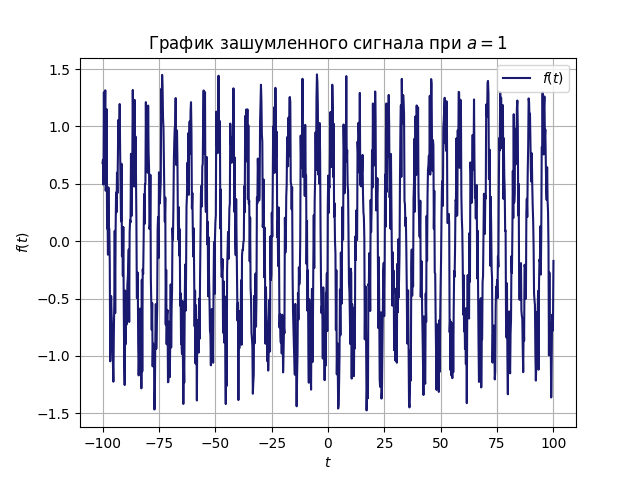
\includegraphics[width=0.78\linewidth]{pic1/n_1.png}}
\caption{Зашумленный график.}
\center{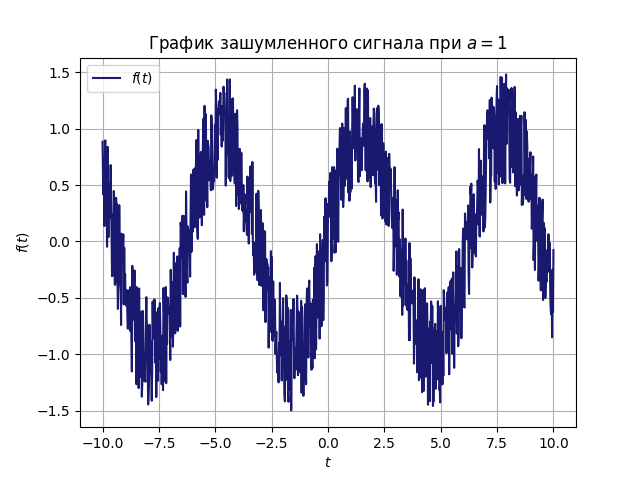
\includegraphics[width=0.78\linewidth]{pic1/n_2.png}}
\caption{Часть зашумленного графика.}
\end{figure}


\newpage
\subsection{Численная производная}
Найдем \textit{численную производную} от зашумленного сигнала, используя формулу поэлементного дифференцирования

\begin{equation}
\frac{y(k+1) - y(k)}{dt}
\end{equation}

\begin{figure}[h!]
\center{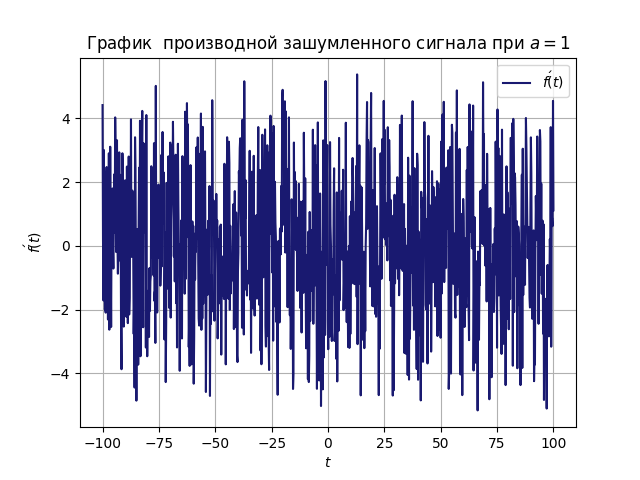
\includegraphics[width=1\linewidth]{pic1/n_d_1.png}}
\caption{Численная производная зашумленного графика функции при $a=1$ на полном промежутке $[-100; 100]$.}
\end{figure}

\begin{figure}[h!]
\center{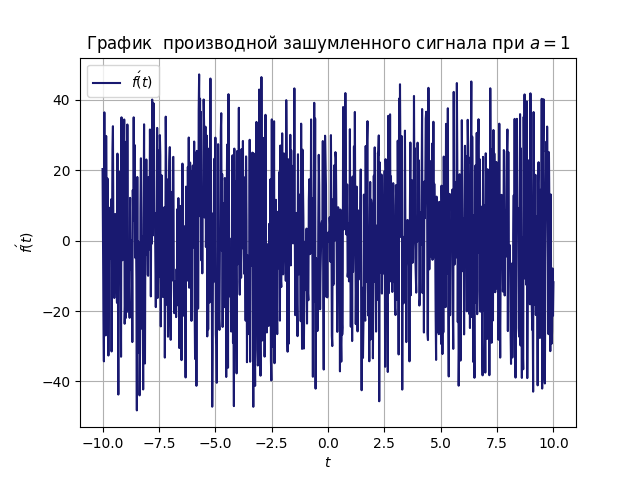
\includegraphics[width=0.78\linewidth]{pic1/n_d_2.png}}
\caption{Численная производная зашумленного графика функции при $a=1$.}
\center{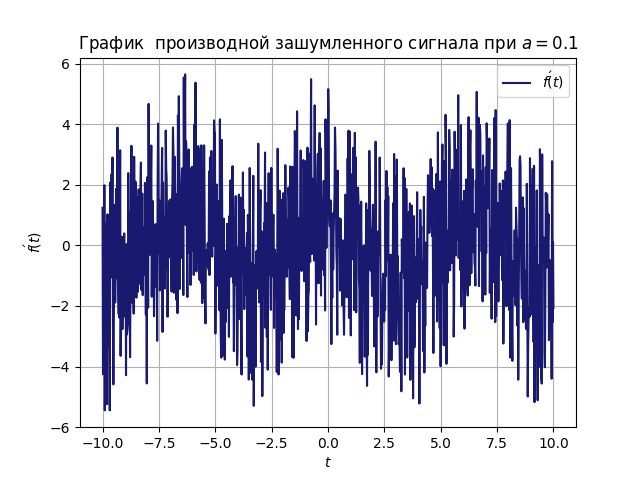
\includegraphics[width=0.78\linewidth]{pic1/n_d_3.png}}
\caption{Численная производная зашумленного графика функции при $a=0.1$.}
\end{figure}


Несмотря на то, что исходный график функции можно узнать при добавлении шума с коэффициентом $a=1$, график численной производной в этом случае практически неузнаваем (рисунки 5-6), но при $a=0.1$ очертания косинуса хорошо заметны и на графике численной производной (рисунок 7).


\newpage
\subsection{Спектральная производная}

Найдем \textit{спектральную производную} от зашумленного сигнала. Для этого с помощью численного интегрирования (\textit{numpy.trapz}) найдем Фурье-образ сигнала и домножим его на $\omega i$, так как $F\{ f'(t)\} = \omega i F\{ f(t)\}$, для того, чтобы получить Фурье-образ производной. \\
После чего выполним обратное преобразование Фурье для получения спектральной производной.

\begin{figure}[h!]
\center{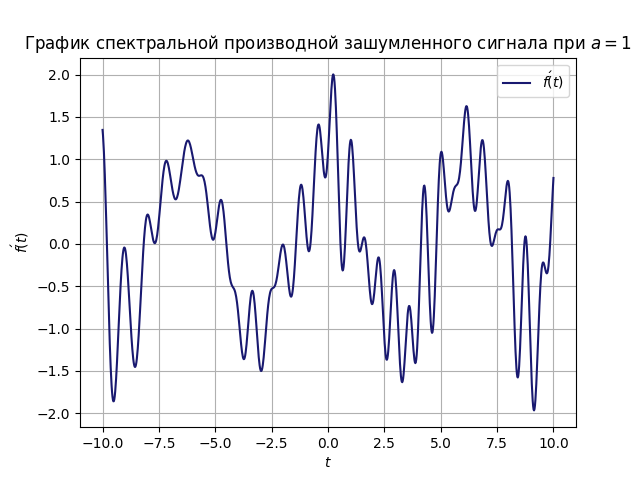
\includegraphics[width=1\linewidth]{pic1/sp_d_10_1.png}}
\caption{Спектральная производная зашумленного графика функции при $a=1$.}
\end{figure}

\begin{figure}[h!]
\center{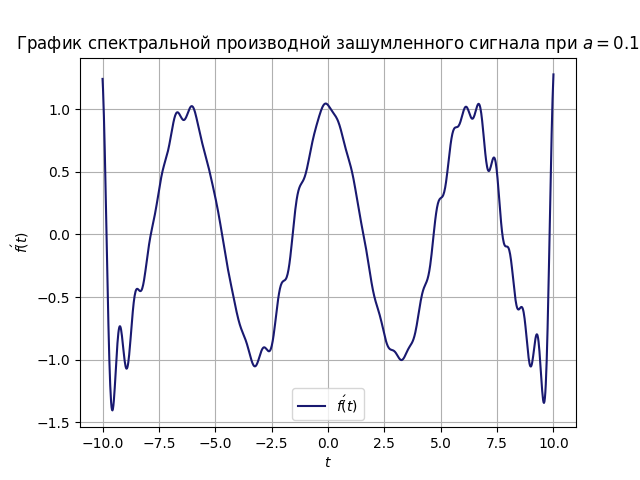
\includegraphics[width=0.78\linewidth]{pic1/sp_d_10_0.1.png}}
\caption{Спектральная производная зашумленного графика функции при $a=0.1$.}
\center{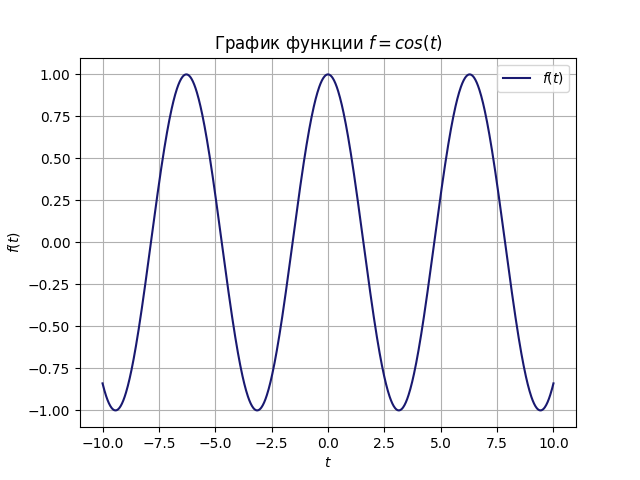
\includegraphics[width=0.78\linewidth]{pic1/true_d.png}}
\caption{График истинной производной.}
\end{figure}

\begin{figure}[h!]
\center{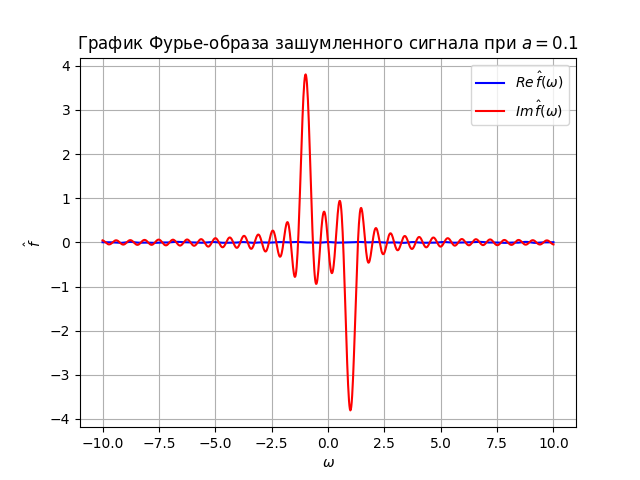
\includegraphics[width=0.78\linewidth]{pic1/im_10_0.1.png}}
\caption{График Фурье-образа зашумленной функции при $a=0.1$.}
\center{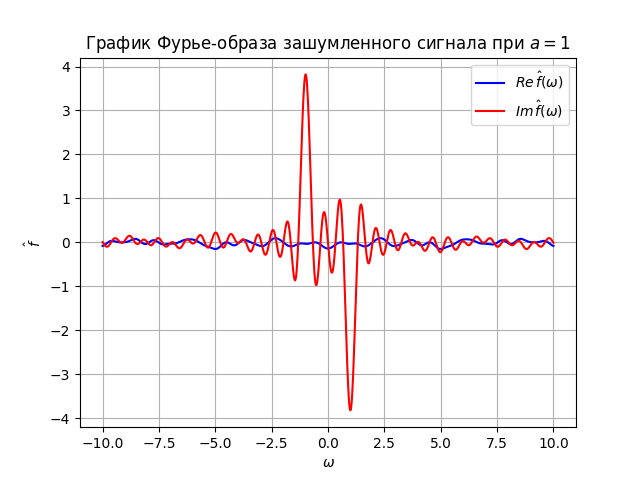
\includegraphics[width=0.78\linewidth]{pic1/im_10_1.png}}
\caption{График Фурье-образа зашумленной функции при $a=1$.}
\end{figure}


На промежутке $[-10; 10]$ графика заметно, что спектральная производная сильнее приближает точную производную $f'(t) = \cos(t)$ (рисунок 10) исходного графика функции по сравнению с численной производной. Причем как в случае $a=1$, так и $a=0.1$. Спектральная производная отличается меньщим количеством шумов, чем численная.\\
\textbf{Вывод:} применение Фурье-преобразования может помочь получить более точную производную функции зашумленного сигнала.






\newpage
\section{Задание. Линейные фильтры.}

Рассмотрим сигнал $$u = g + b \cdot (rand(size(t)) - 0.5) + c \cdot \sin (d \cdot t)$$
и выполним фильтрацию указанного сигнала, используя линейные фильтры.\\
 Сигнал $g(t)$ также перепишем из лабораторной 3: зададимся числами $a=1$, $t_1 = 0$, $t_2 = 2$ и рассмотрим функцию $g(t) = a$ при $t \in [t_1, t_2]$ и $g(t) = 0$ при других $t$.

\begin{figure}[h!]
\center{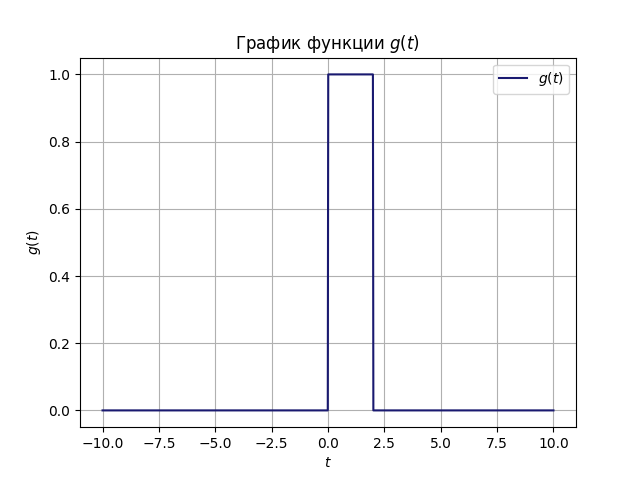
\includegraphics[width=1\linewidth]{pic2/g.png}}
\caption{Исходный график функции $g(t)$.}
\end{figure}

\begin{figure}[h!]
\center{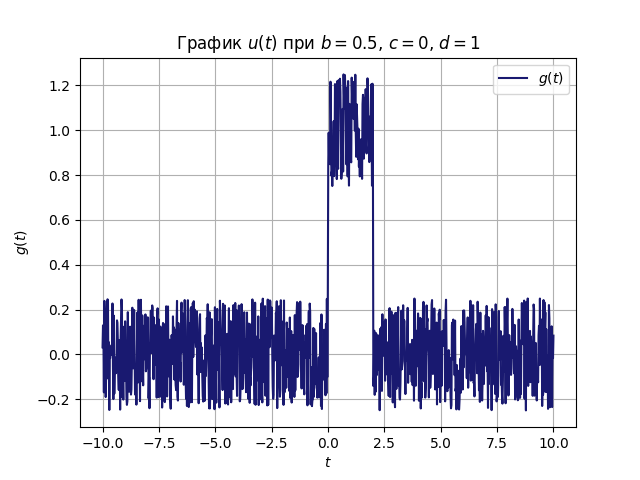
\includegraphics[width=1\linewidth]{pic2/u_0.5_0_1.png}}
\caption{График $u(t)$ при $b=0.5$, $c = 0$, $d = 1$.}
\end{figure}


\newpage
\subsection{Фильтр первого порядка.}
Пусть $c= 0$. Зададим постоянную времени $T > 0$ и пропустим сигнал $u$ через линейный фильтр первого порядка

\begin{equation}
W_1 (p) = \frac{1}{Tp + 1}
\end{equation}



\begin{figure}[h!]
\center{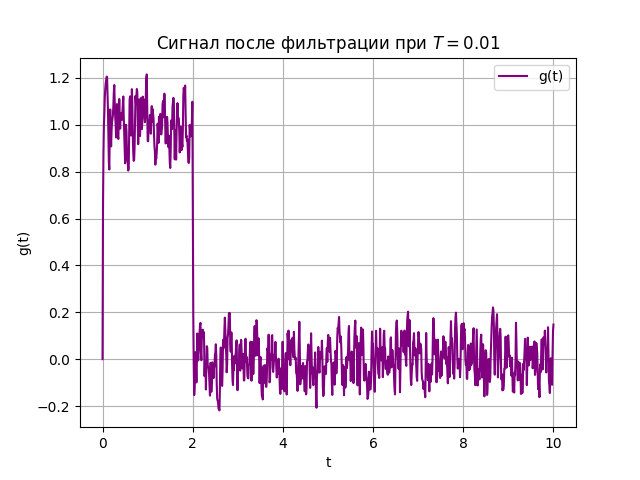
\includegraphics[width=0.78\linewidth]{pic2/f_1_0.01.png}}
\caption{График после фильтрации при $T = 0.01$.}
\center{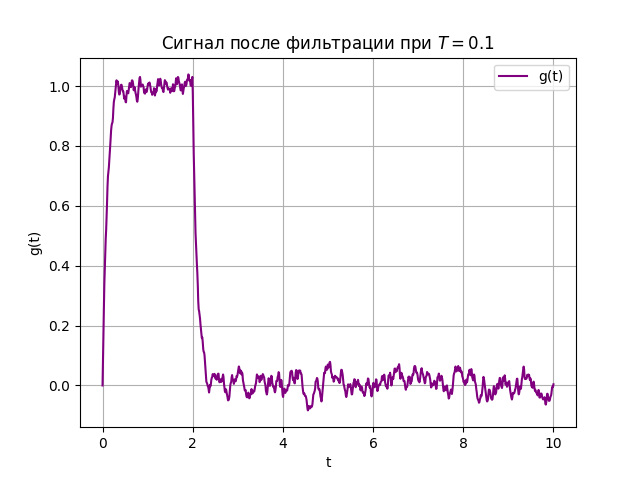
\includegraphics[width=0.78\linewidth]{pic2/f_1_0.1.png}}
\caption{График после фильтрации при $T = 0.1$.}
\end{figure}

Заметим, что при малом значении параметра $T$ шумы из сигнала практически не убираются (рисунок 15), но при увеличении значения коэффициента $T$ график становится более гладким (рисунок 16).\\


\begin{figure}[h!]
\center{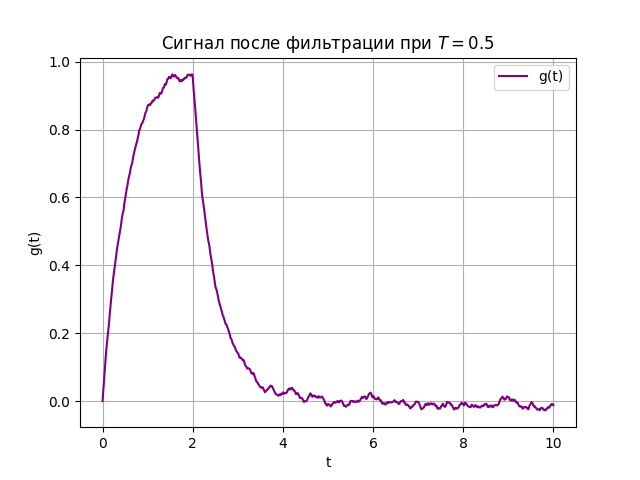
\includegraphics[width=0.78\linewidth]{pic2/f_1_0.5.png}}
\caption{График после фильтрации при $T = 0.5$.}
\center{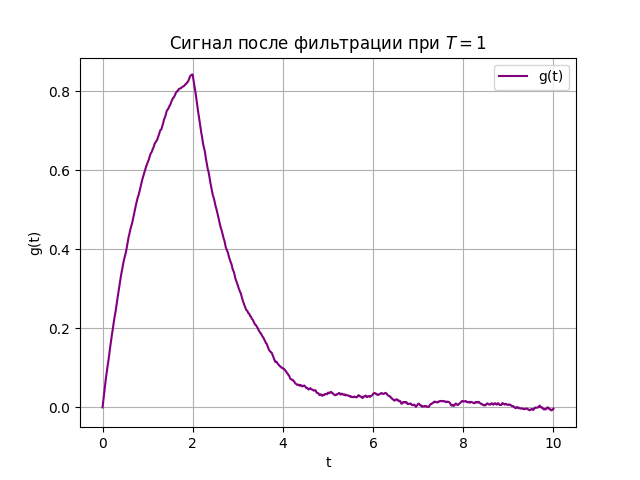
\includegraphics[width=0.78\linewidth]{pic2/f_1_1.png}}
\caption{График после фильтрации при $T = 1$.}
\end{figure}
\,\\
\\
\\
\\
При дальнейшем увеличении значения параметра $T$, начиная с $T= 1$ (рисунок 18), теряется точность передаваемого сигнала.
\subsubsection{Сравнительные графики исходного, зашумленного и сигнала после фильтрации}
\begin{figure}[h!]
\center{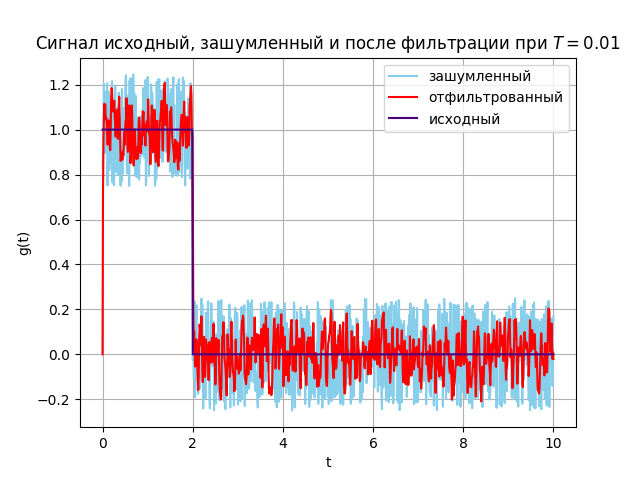
\includegraphics[width=1\linewidth]{pic2/trio_0.01.png}}
\caption{Сравнительные графики при $T = 0.01$.}
\end{figure}

Далее, на рисунках 19-22 представлены сравнительные графики исходного сигнала $g(t)$, сигнала с шумами $u(t)$ и сигнала после фильтрации при разных значениях параметра $T$.

\begin{figure}[h!]
\center{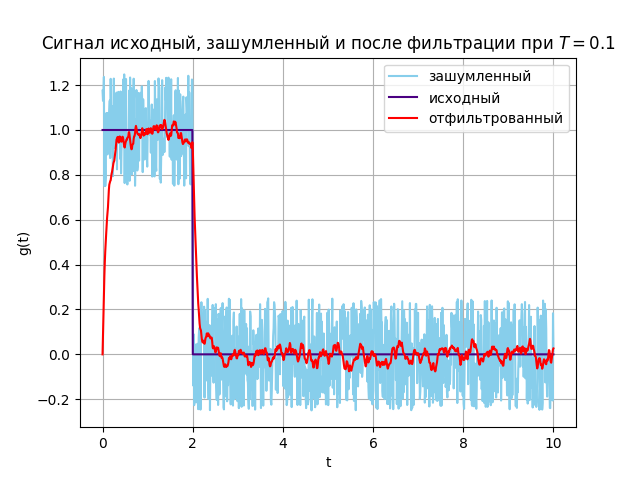
\includegraphics[width=0.78\linewidth]{pic2/trio_0.1.png}}
\caption{Сравнительные графики при $T = 0.1$.}
\center{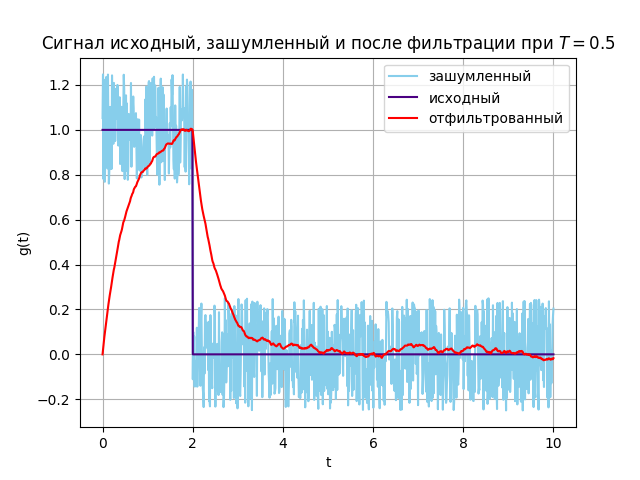
\includegraphics[width=0.78\linewidth]{pic2/trio_0.5.png}}
\caption{Сравнительные графики при $T = 0.5$.}
\end{figure}

\begin{figure}[h!]
\center{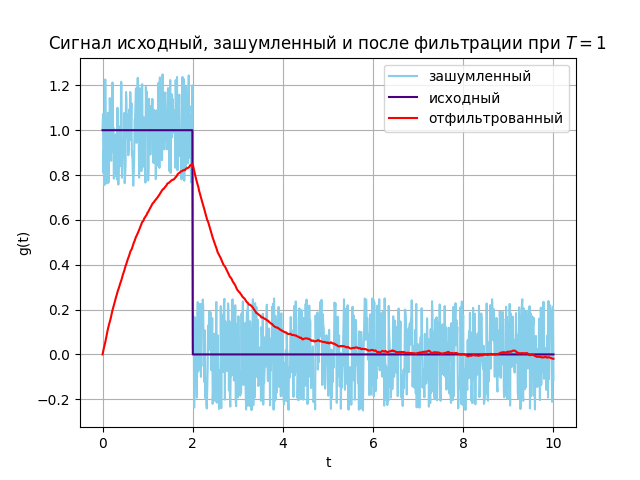
\includegraphics[width=1\linewidth]{pic2/trio_1.png}}
\caption{Сравнительные графики при $T = 1$.}
\end{figure}
\, \\
\\
\\
\\
\\
\\
Наибольшее сходство фильтрованного сигнала с исходным достигается при $T=0.1$, в чем можно убедиться, сравнив результаты, представленные на рисунках 19 - 22.\\
\subsubsection{Модули Фурье-образов}
Модули Фурье-образов исходного и фильтрованного сигналов наиболее близки друг к другу при небольших значениях $T$, например, $T=0.01$ (рисунок 23) и $T=0.1$ (рисунок 24). При дальнейшем возрастании параметра $T$ модуль Фурье-образа фильтрованного сигнала становится все более гладким и отличным от исходного сигнала. Фильтр избавляет от более высоких частот и чем выше параметр $T$ тем ниже модуль подавляемых частот.

\begin{figure}[h!]
\center{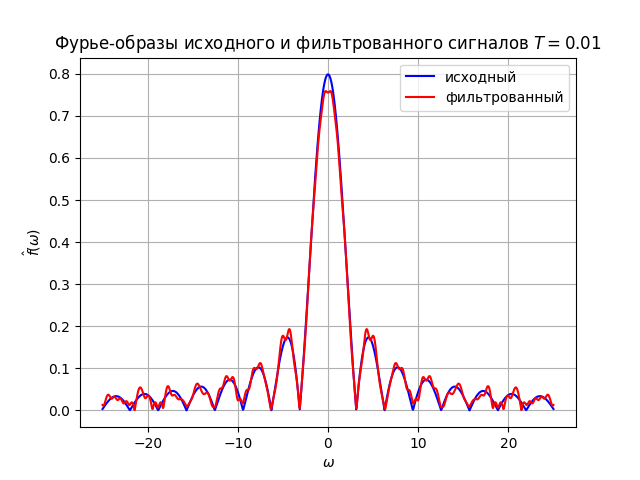
\includegraphics[width=0.78\linewidth]{pic2/mod_im_0.01.png}}
\caption{Модули Фурье-образов сигналов при $T = 0.01$.}
\center{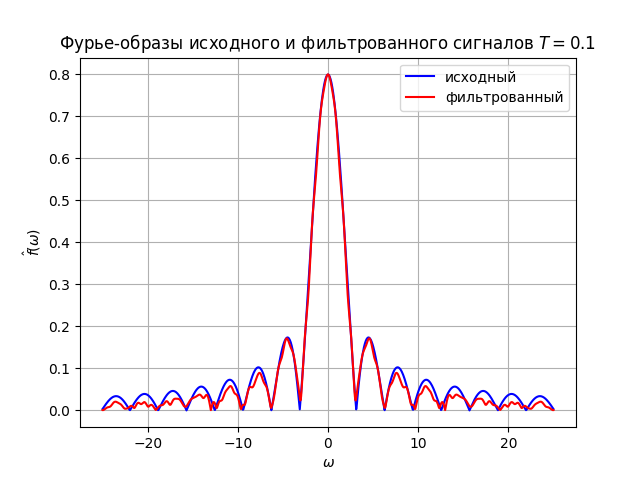
\includegraphics[width=0.78\linewidth]{pic2/mod_im_0.1.png}}
\caption{Модули Фурье-образов сигналов при $T = 0.1$.}
\end{figure}


\begin{figure}[h!]
\center{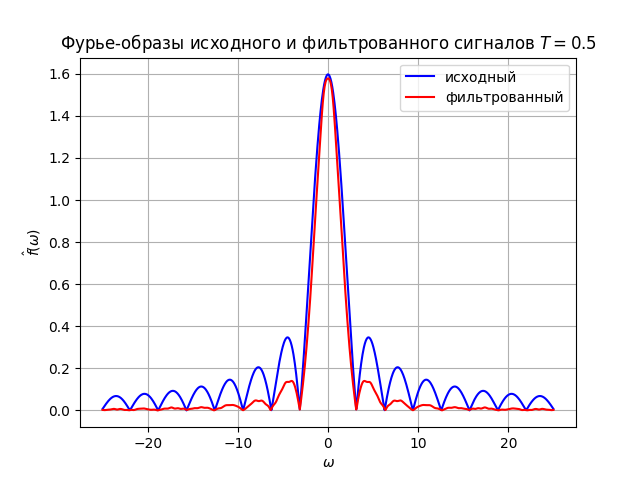
\includegraphics[width=0.78\linewidth]{pic2/mod_im_0.5.png}}
\caption{Модули Фурье-образов сигналов при $T = 0.5$.}
\center{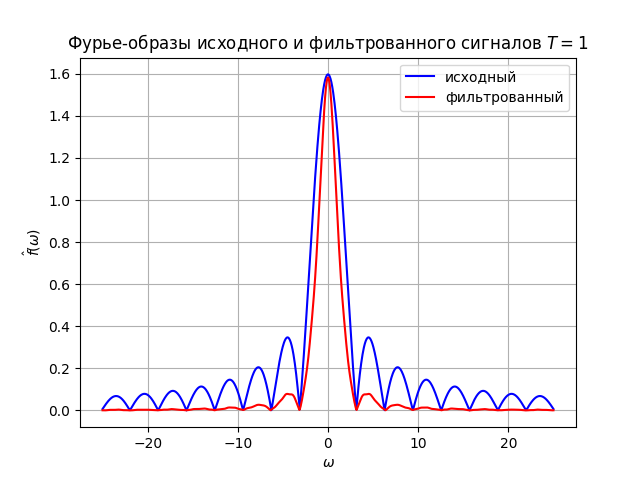
\includegraphics[width=0.78\linewidth]{pic2/mod_im_1.png}}
\caption{Модули Фурье-образов сигналов при $T = 1$.}
\end{figure}
\, \\
\subsubsection{Амплитудно-частотные характеристики фильтра}
Построим также графики амплитудно-частотной характеристики линейного фильтра первого порядка.
\begin{figure}[h!]
\center{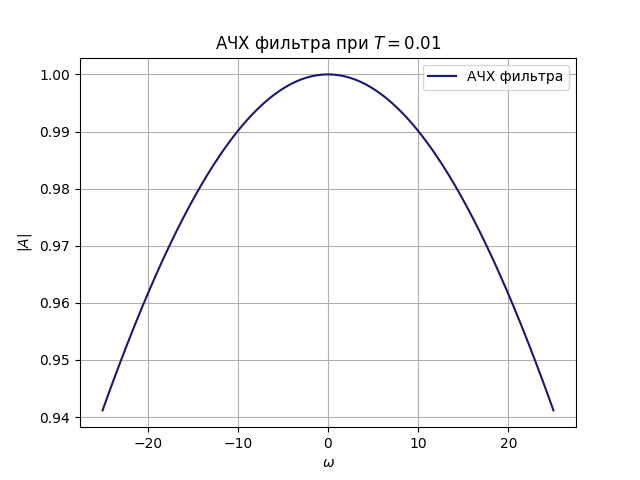
\includegraphics[width=1\linewidth]{pic2/zpk_1_0.01.png}}
\caption{АЧХ при $T = 0.01$.}
\end{figure}

Если опустить перпендикуляры на ось абсцисс из точек пересечения графика АЧХ с прямой $|A| = \frac{1}{\sqrt{2}} \simeq 0.7$, получим значения частот, выше которых частоты подавляются фильтром. Нетрудно заметить, что в случае $T=0.01$ подавляются очень высокие значения частот, поэтому разницы между сигнала с шумом и фильтрованным сигналом практически нет (рисунок 19). Наилучший результат был достигнут при $T=0.1$, в этом случает подавляются частоты выше $7$ по модулю, при увеличении значения $T$ (рисунки 29-30) диапазон подавляемых частот становится настолько большим, что теряется сходство исходного сигнала и сигнала после фильтрации.

\begin{figure}[h!]
\center{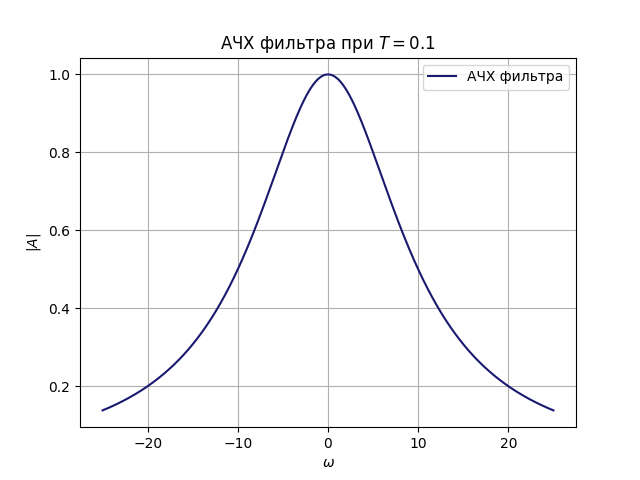
\includegraphics[width=0.78\linewidth]{pic2/zpk_1_0.1.png}}
\caption{АЧХ при $T = 0.1$.}
\center{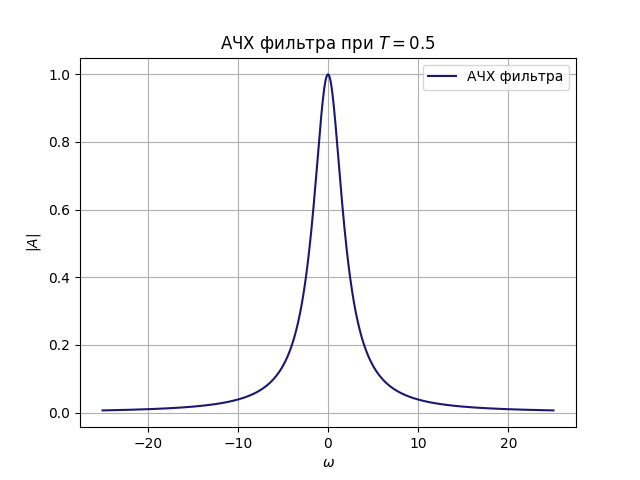
\includegraphics[width=0.78\linewidth]{pic2/zpk_1_0.5.png}}
\caption{АЧХ при $T = 0.5$.}
\end{figure}

\begin{figure}[h!]
\center{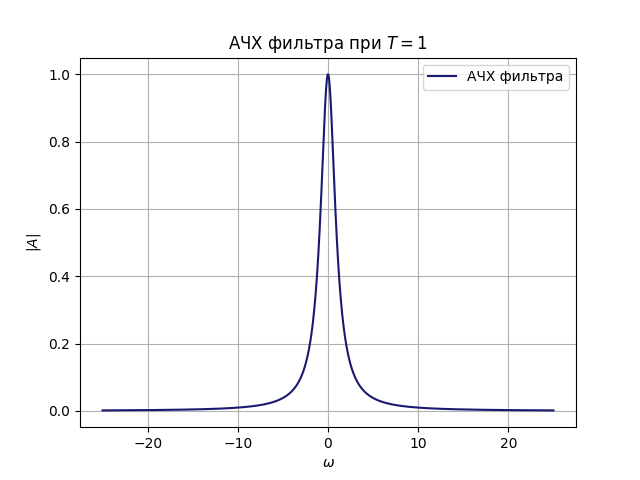
\includegraphics[width=1\linewidth]{pic2/zpk_1_1.png}}
\caption{АЧХ при $T = 1$.}
\end{figure}

\subsubsection{Влияние параметра $a$}
Рассмотрим, как изменится результат фильтрации при $a = \{0.1, 0.5, 1, 2\}$ при $T=\{ 0.01, 0.1, 0.5, 1\}$.\\

Параметр $a$ существенно не влияет на успешность фильтрации: при $T=0.01$ -- очистки от шумов практически не происходит, при $T=1$ график получается слишком пологим, а наиболее оптимальный результат немного отличается, например, при $a=0.1$ лучшее значение параметра $T=0.5$, для значений $a=0.5$, $a=1$, $a=2$ подходит $T=0.1$.

\begin{figure}[h!]
\begin{minipage}[h!]{0.47\linewidth}
\center{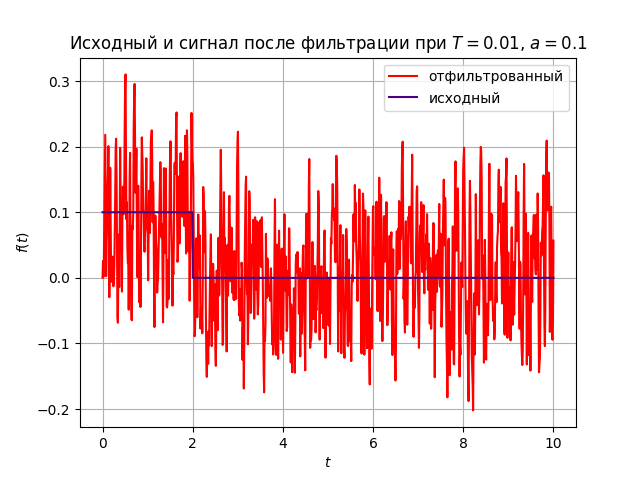
\includegraphics[width=1\linewidth]{pic2/a_0.1_0.01}} a) \\
\end{minipage}
\hfill
\begin{minipage}[h!]{0.47\linewidth}
\center{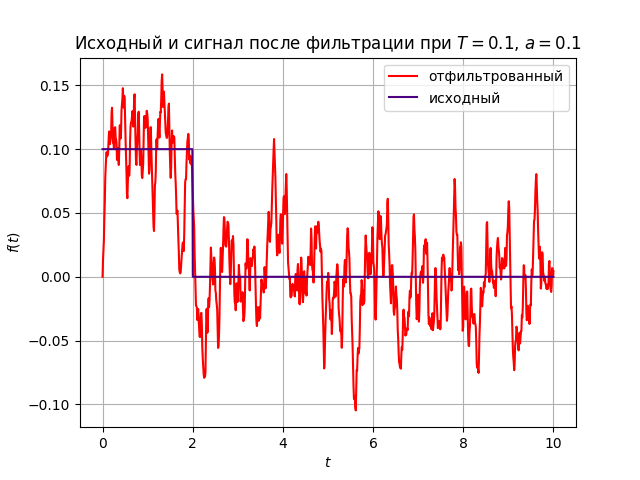
\includegraphics[width=1\linewidth]{pic2/a_0.1_0.1}} \\b)
\end{minipage}
\vfill
\begin{minipage}[h!]{0.47\linewidth}
\center{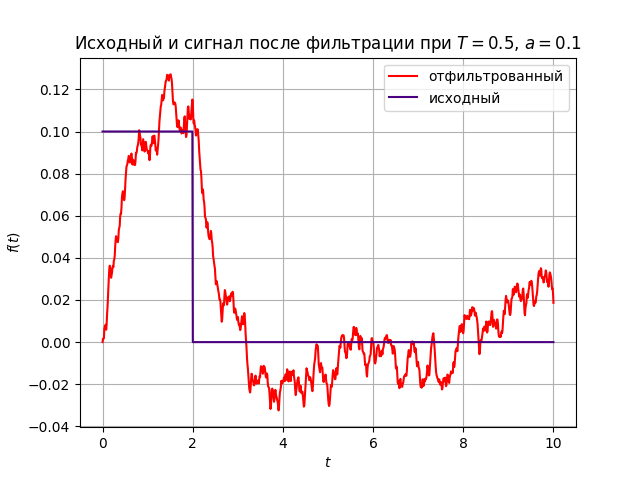
\includegraphics[width=1\linewidth]{pic2/a_0.1_0.5}} c) \\
\end{minipage}
\hfill
\begin{minipage}[h!]{0.47\linewidth}
\center{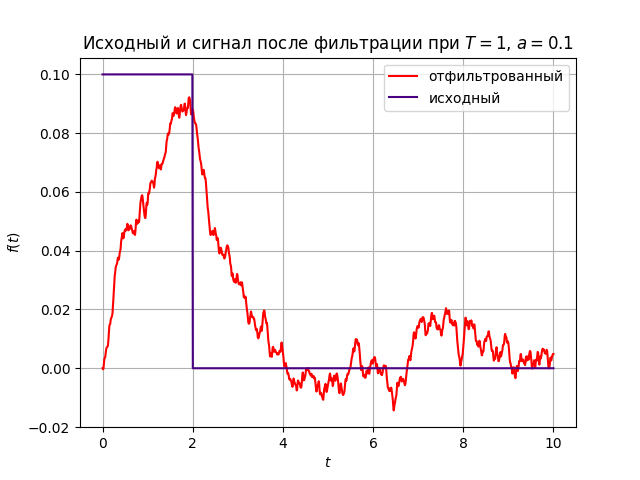
\includegraphics[width=1\linewidth]{pic2/a_0.1_1}} d) \\
\end{minipage}
\caption{Сравнительные графики исходного и фильтрованного сигналов для $a=0.1$ при: a) $T=0.01$, b)
$T=0.1$, c) $T=0.5$, d) $T=1$.}
\end{figure}

\begin{figure}[h!]
\begin{minipage}[h!]{0.47\linewidth}
\center{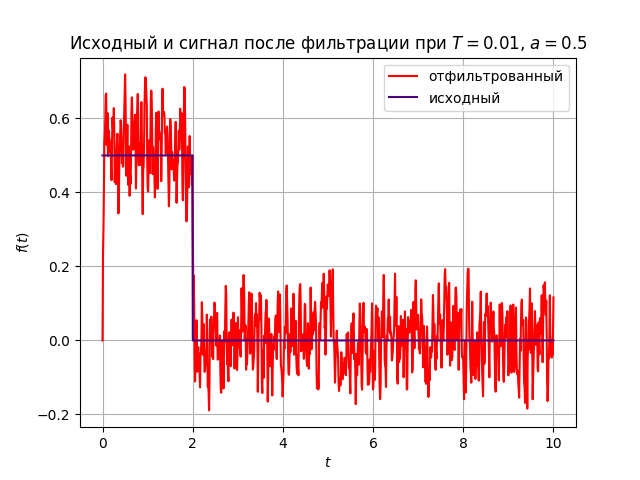
\includegraphics[width=1\linewidth]{pic2/a_0.5_0.01}} a) \\
\end{minipage}
\hfill
\begin{minipage}[h!]{0.47\linewidth}
\center{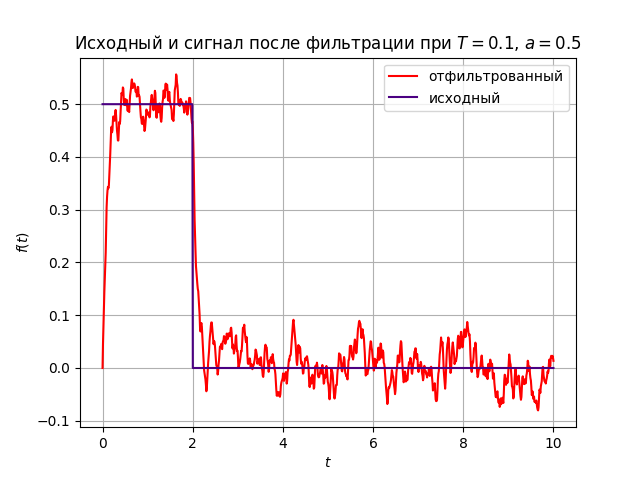
\includegraphics[width=1\linewidth]{pic2/a_0.5_0.1}} \\b)
\end{minipage}
\vfill
\begin{minipage}[h!]{0.47\linewidth}
\center{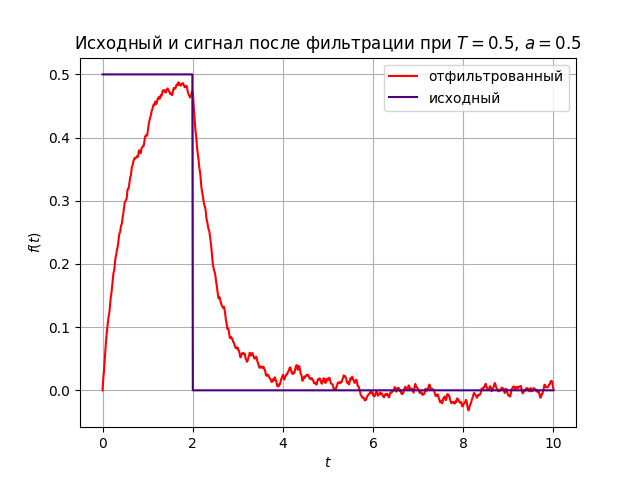
\includegraphics[width=1\linewidth]{pic2/a_0.5_0.5}} c) \\
\end{minipage}
\hfill
\begin{minipage}[h!]{0.47\linewidth}
\center{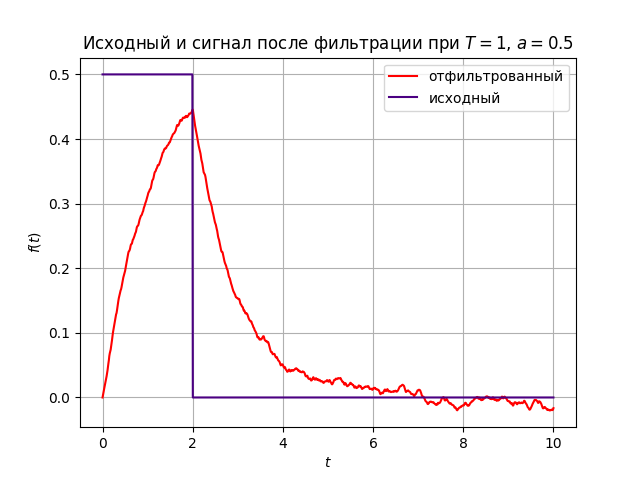
\includegraphics[width=1\linewidth]{pic2/a_0.5_1}} d) \\
\end{minipage}
\caption{Сравнительные графики исходного и фильтрованного сигналов для $a=0.5$ при: a) $T=0.01$, b)
$T=0.1$, c) $T=0.5$, d) $T=1$.}
\end{figure}

\begin{figure}[h!]
\begin{minipage}[h!]{0.47\linewidth}
\center{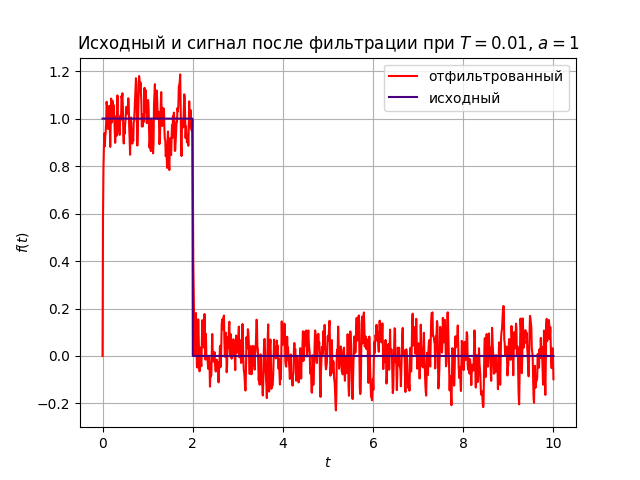
\includegraphics[width=1\linewidth]{pic2/a_1_0.1}} a) \\
\end{minipage}
\hfill
\begin{minipage}[h!]{0.47\linewidth}
\center{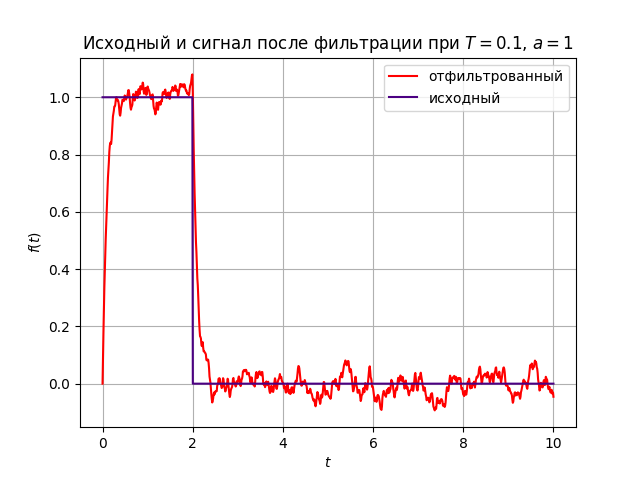
\includegraphics[width=1\linewidth]{pic2/a_1_t_0.1}} \\b)
\end{minipage}
\vfill
\begin{minipage}[h!]{0.47\linewidth}
\center{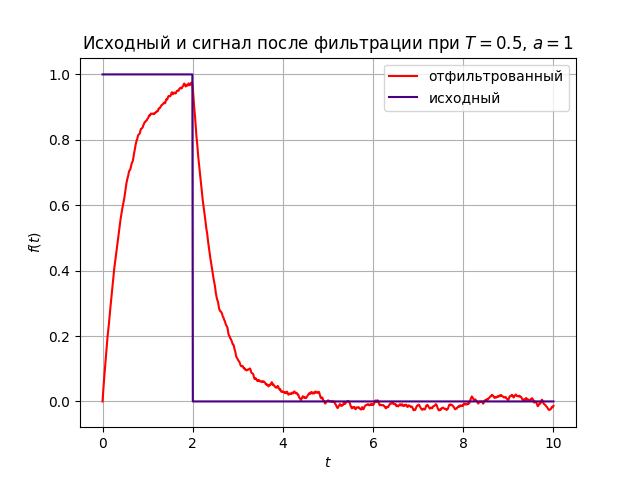
\includegraphics[width=1\linewidth]{pic2/a_1_t_0.5}} c) \\
\end{minipage}
\hfill
\begin{minipage}[h!]{0.47\linewidth}
\center{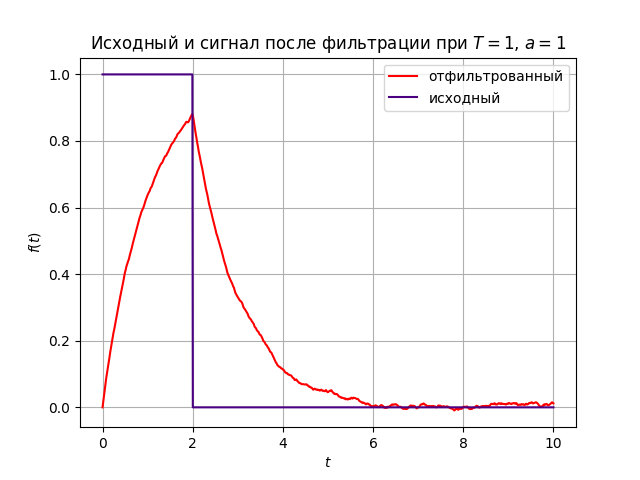
\includegraphics[width=1\linewidth]{pic2/a_1_t_1}} d) \\
\end{minipage}
\caption{Сравнительные графики исходного и фильтрованного сигналов для $a=1$ при: a) $T=0.01$, b)
$T=0.1$, c) $T=0.5$, d) $T=1$.}
\end{figure}

\begin{figure}[h!]
\begin{minipage}[h!]{0.47\linewidth}
\center{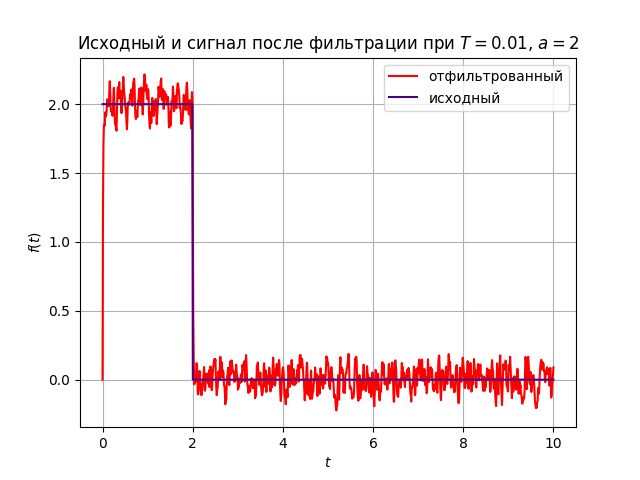
\includegraphics[width=1\linewidth]{pic2/a_2_t_0.01}} a) \\
\end{minipage}
\hfill
\begin{minipage}[h!]{0.47\linewidth}
\center{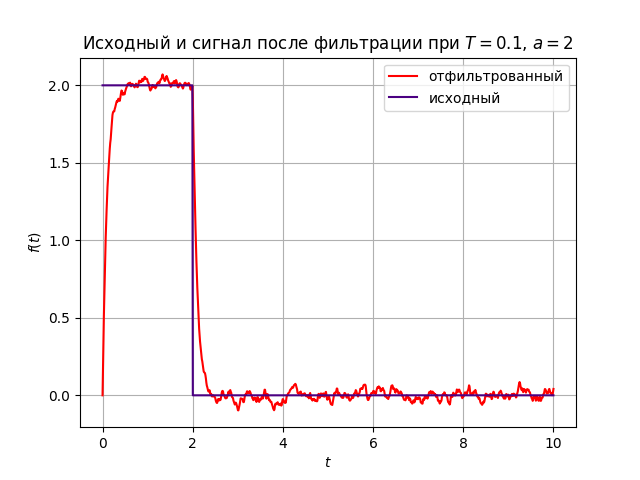
\includegraphics[width=1\linewidth]{pic2/a_2_t_0.1}} \\b)
\end{minipage}
\vfill
\begin{minipage}[h!]{0.47\linewidth}
\center{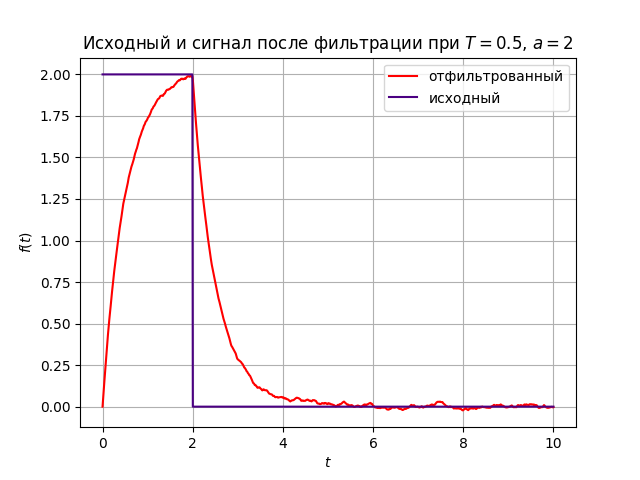
\includegraphics[width=1\linewidth]{pic2/a_2_t_0.5}} c) \\
\end{minipage}
\hfill
\begin{minipage}[h!]{0.47\linewidth}
\center{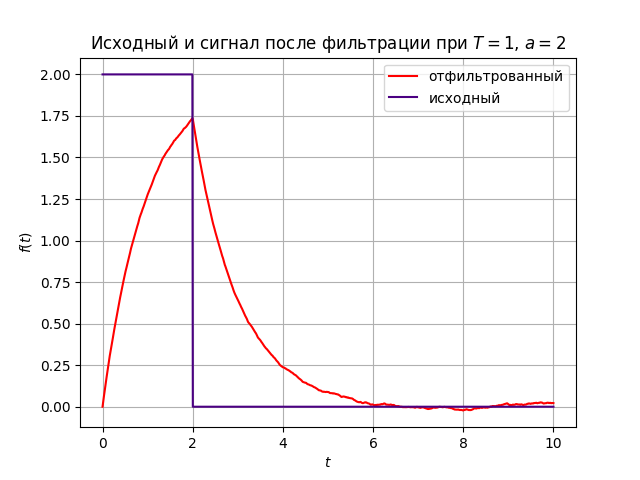
\includegraphics[width=1\linewidth]{pic2/a_2_t_1}} d) \\
\end{minipage}
\caption{Сравнительные графики исходного и фильтрованного сигналов для $a=2$ при: a) $T=0.01$, b)
$T=0.1$, c) $T=0.5$, d) $T=1$.}
\end{figure}




\,
\\\\\\
\\
\\
\\
\\
\\
\\
\\
\\
\\
\\
\\
\\
\\

\newpage
\,
\newpage
\,
\newpage
\subsection{Специальный фильтр}









\newpage
\section{Задание. Сглаживание биржевых линий.}


\newpage
Для визуализации был написан код на языке \textit{Python}. \\
Код расположен на \href{https://github.com/a-nechaeva/practical_Linal/tree/main/lab4}{\textbf{GitHub}}.
\end{document}













